
\documentclass[11pt,a4paper]{article}

% --------------------------------------------------
% PAQUETES
% --------------------------------------------------

\usepackage[utf8]{inputenc}
\usepackage[T1]{fontenc}
\usepackage[spanish]{babel}

\usepackage{geometry}
\geometry{margin=2.3cm}

\usepackage{graphicx}
\usepackage{float}
\usepackage{booktabs}
\usepackage{amsmath}
\usepackage{hyperref}
\usepackage{caption}

% Carátula gráfica
\usepackage[graf,intVert]{caratula}

% --------------------------------------------------
% DATOS DE LA CARÁTULA
% --------------------------------------------------

\materia{Laboratorio de Datos}
\titulo{Trabajo Práctico 2}
\subtitulo{Análisis y experimentación con modelos}
\fecha{1 de noviembre de 2026}

% Reemplazar por los datos reales del grupo.
\grupo{Normalizados}

\integrante{Ayala Ignacio}{196/25}{ayalanacho11@gmail.com}
\integrante{Della Bonzana Lara}{563/25}{dellabonzanalara@gmail.com}
\integrante{Posse Lucila}{618/25}{lucila.posse@gmail.com}
\integrante{Ventroni Milena}{647/25}{milena.ventroni@gmail.com}
% Agregar una línea \integrante por cada integrante.

% --------------------------------------------------
% INICIO DEL DOCUMENTO
% --------------------------------------------------

\begin{document}

\maketitle

% ==================================================
\section{Introducción y análisis exploratorio}
% ==================================================

El presente trabajo tiene como objetivo analizar y evaluar distintos 
modelos de clasificación supervisada a partir de un conjunto de imágenes
pertenecientes al dataset Quick, Draw! de Google. Buscamos estudiar cómo
la selección de atributos y de hiperparámetros influye en el desempeño 
de los clasificadores y, particularmente, cómo estimar su capacidad para
realizar predicciones sobre imágenes no utilizadas durante el entrenamiento.
Cada imagen está representada por 784 atributos, correspondientes a los píxeles 
de una matriz de $28 \times 28$, y pertenece a una de diez clases posibles.

Para llevar a cabo el trabajo, realizamos inicialmente un análisis exploratorio de 
los datos, enfocado en estudiar la variabilidad de los atributos y las similitudes 
entre imágenes de una misma clase y de clases diferentes.

A partir de este análisis, abordamos dos problemas de clasificación. En primer lugar, 
buscamos distinguir imágenes de cuadrados y casas mediante el algoritmo de los (k) 
vecinos más cercanos (KNN), evaluando cómo la selección de atributos y la cantidad de 
vecinos afectan el desempeño del modelo. Luego, trabajamos con las diez clases utilizando 
árboles de decisión. Para seleccionar sus hiperparámetros recurrimos a la validación cruzada 
y utilizamos un conjunto de control independiente para estimar su capacidad de generalización.


\subsection{Análisis exploratorio}

El conjunto de entrenamiento contiene 30.000 imágenes
etiquetadas, mientras que el conjunto de evaluación cuenta
con 6.030 imágenes sin etiquetar, identificadas mediante
un código único. Comprobamos que los atributos son de tipo
entero y que sus intensidades toman valores entre 0 y 255,
de los cuales encontramos 143 valores distintos. Tampoco
identificamos valores faltantes ni filas duplicadas en
los conjuntos analizados.

Para determinar qué atributos podrían resultar útiles
para distinguir las clases, analizamos la variabilidad
de los píxeles mediante dos mapas de calor. El primero
representa la varianza de las intensidades promedio de
cada píxel entre las distintas clases, mientras que el
segundo muestra el desvío estándar de cada píxel sobre
el conjunto completo.

Como podemos observar en la Figura
\ref{fig:variabilidad_pixeles}, la variabilidad no se
distribuye uniformemente entre los atributos. Las mayores
diferencias entre los promedios de clase se concentran
principalmente cerca del borde superior y del lateral
izquierdo de las imágenes, regiones donde también
encontramos una elevada variabilidad total. En cambio,
las esquinas presentan valores reducidos en ambos gráficos.

También comprobamos que ninguno de los 784 píxeles es
estrictamente constante y que solamente ocho presentan
un desvío estándar inferior a 10.

Estos resultados permiten identificar atributos
potencialmente más relevantes para la clasificación.
Sin embargo, una baja variabilidad total no implica
necesariamente una baja capacidad discriminativa.
Del mismo modo, una variabilidad elevada puede deberse
a diferencias entre dibujos de una misma clase.
Por lo tanto, estos gráficos permiten formular hipótesis
sobre la relevancia de los atributos, pero no garantizan
que eliminar determinados píxeles mejore o preserve
el desempeño de un clasificador.

\begin{figure}[H]
    \centering
    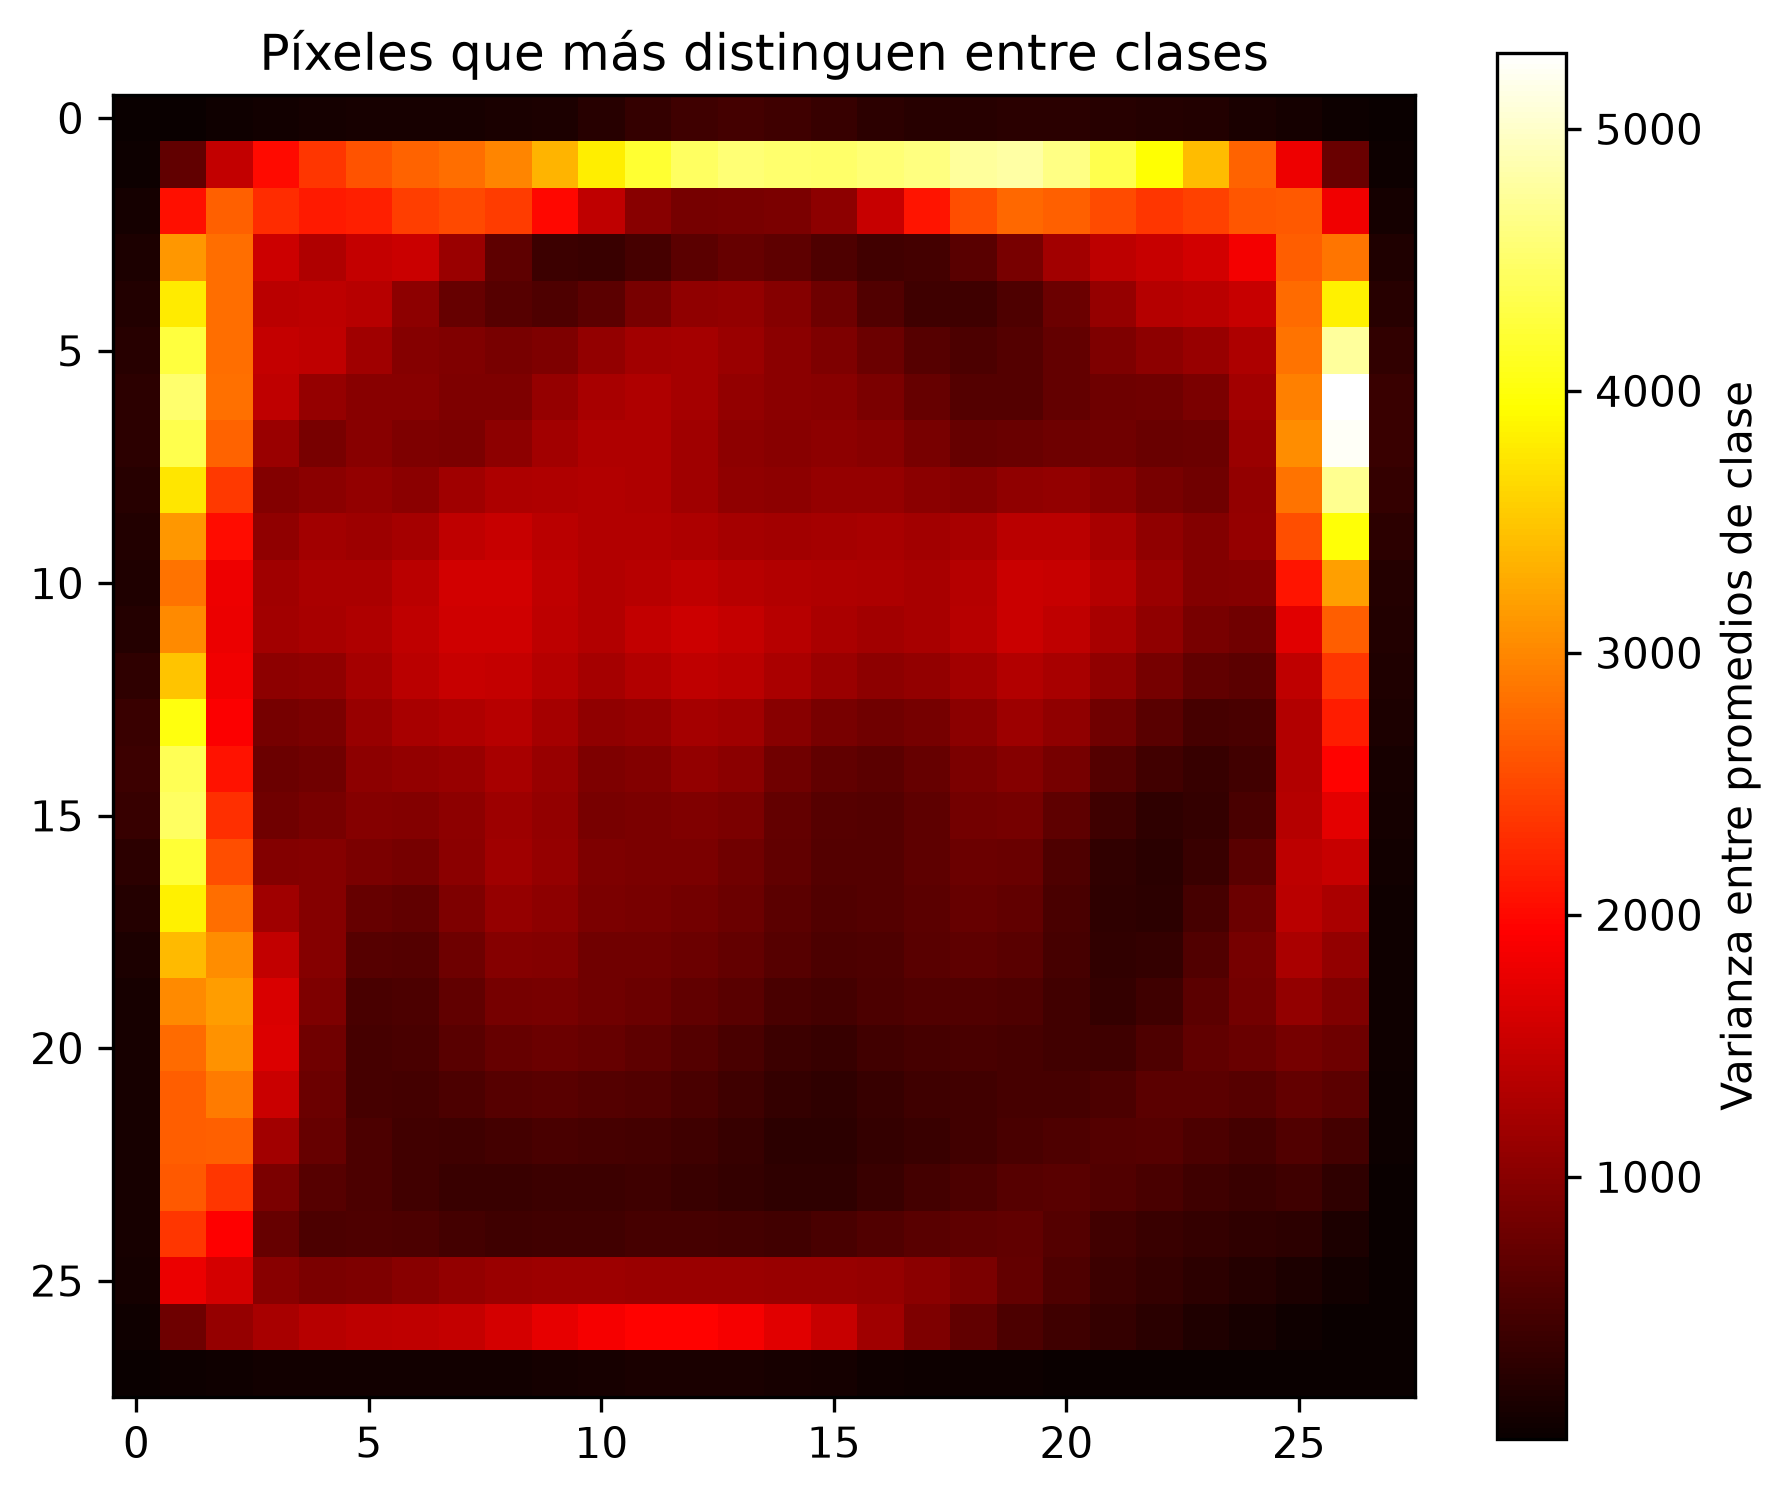
\includegraphics[width=0.46\textwidth]
    {graficos/varianza_entre_clases.png}
    \hfill
    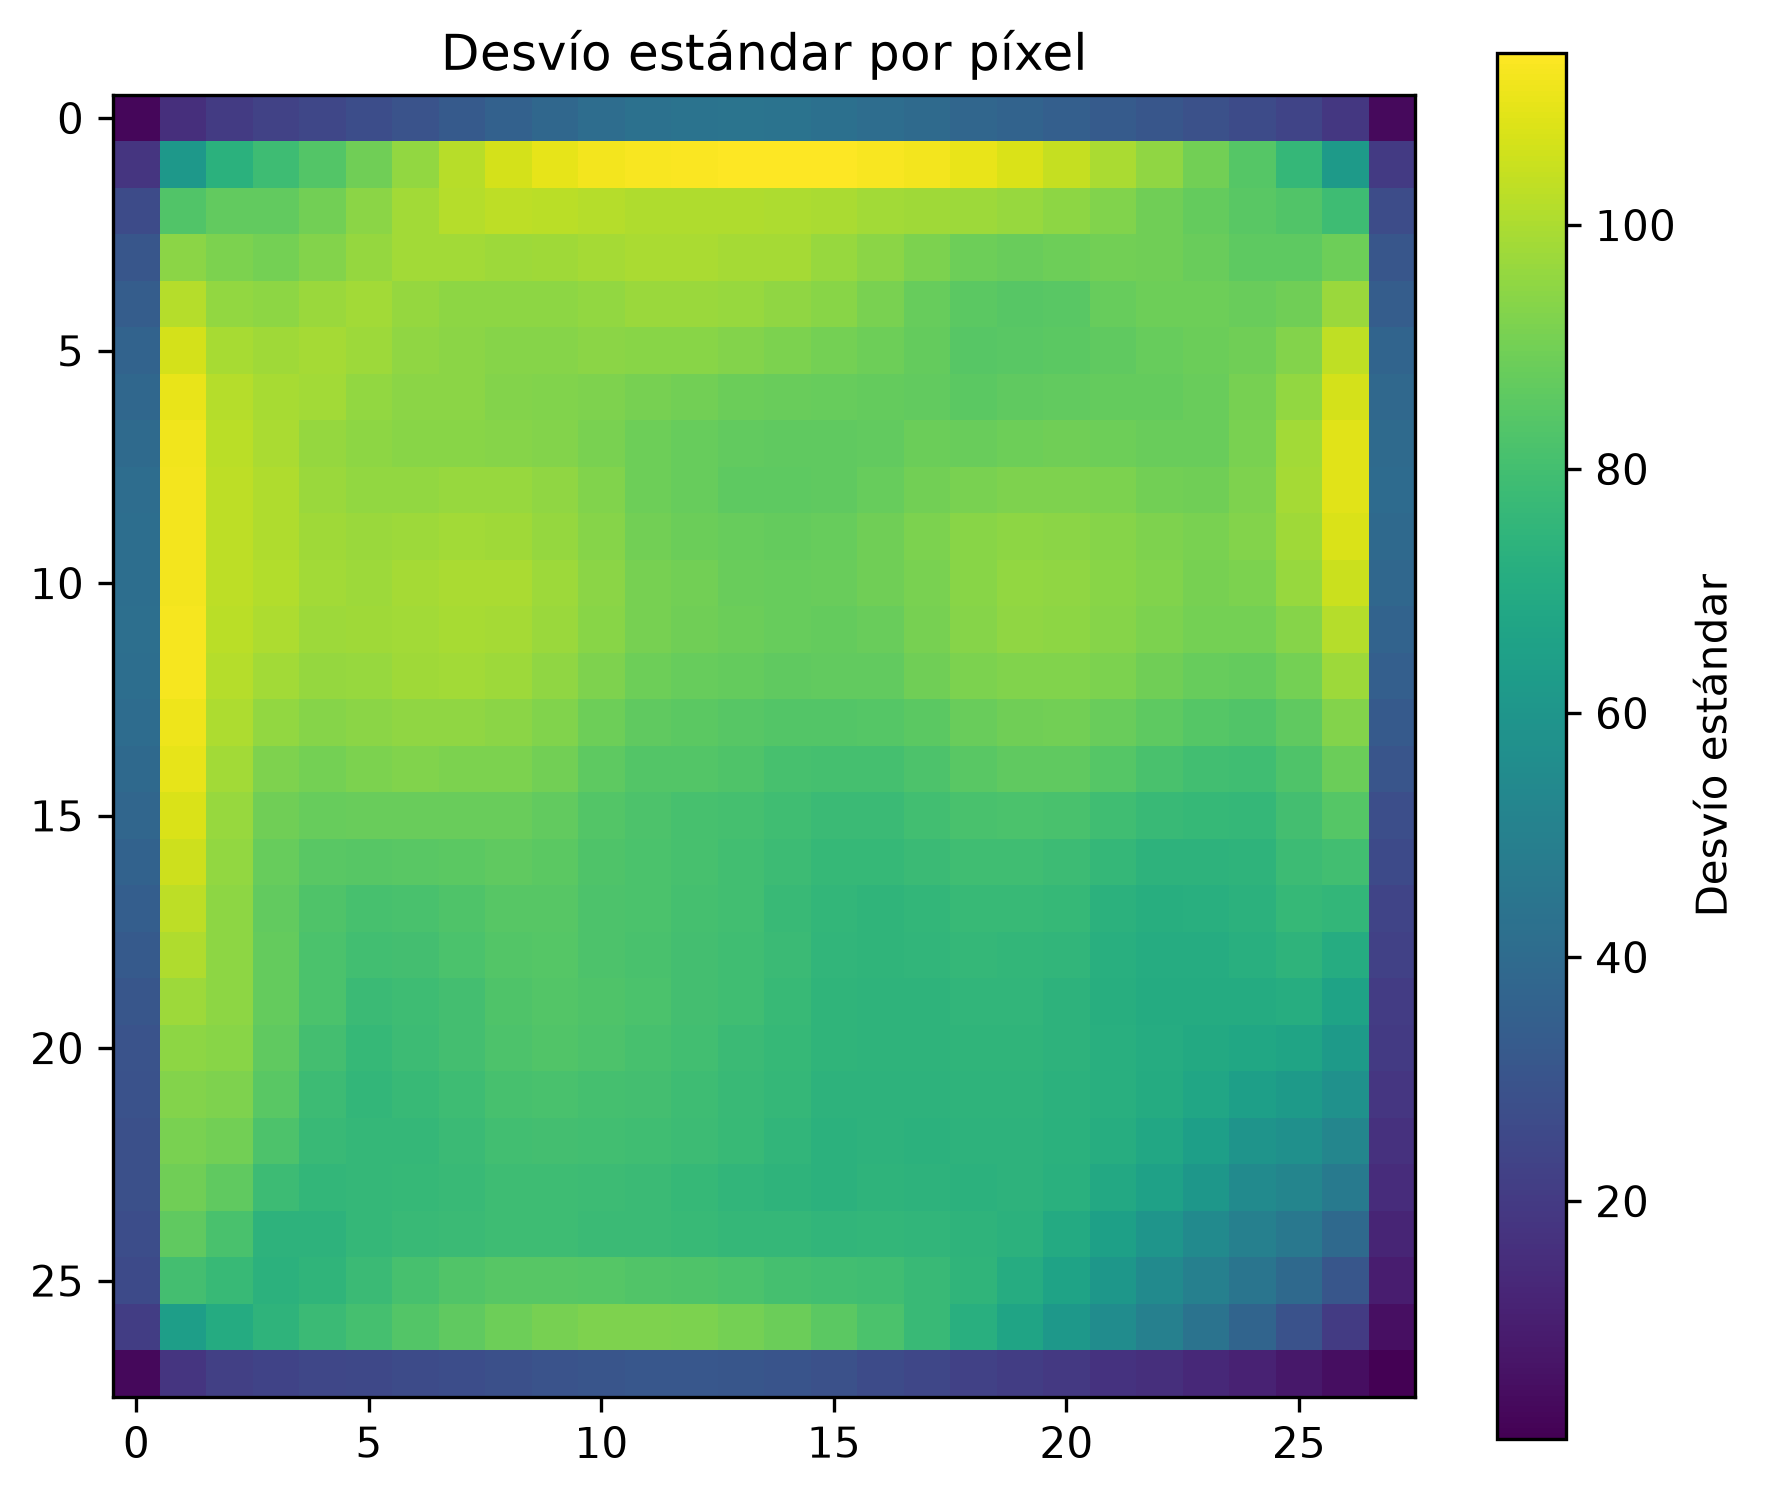
\includegraphics[width=0.46\textwidth]
    {graficos/desvio_total.png}
    \caption{Variabilidad de los atributos.
    Izquierda: varianza de los promedios por clase.
    Derecha: desvío estándar de cada píxel
    sobre el conjunto completo.}
    \label{fig:variabilidad_pixeles}
\end{figure}

Para complementar este análisis, comparamos las
distribuciones de intensidad de dos atributos:
\texttt{pixel194}, que presenta una de las mayores
varianzas entre los promedios de clase, y
\texttt{pixel0}, cuya variabilidad total es reducida.

Como podemos observar en la Figura
\ref{fig:comparacion_pixeles}, las intensidades
del píxel 194 presentan diferencias importantes
entre clases. Mientras que en algunas encontramos
valores elevados y una amplia dispersión, en otras
las intensidades se concentran principalmente en
cero. Esto sugiere que el atributo podría aportar
información relevante para distinguir determinadas
categorías.

En cambio, el píxel 0 presenta intensidades
prácticamente nulas en todas las clases, con
algunos valores atípicos poco frecuentes.
Por lo tanto, este atributo parece tener menor
capacidad para diferenciar las clases por sí solo,
aunque no podemos afirmar que sea completamente
irrelevante al combinarlo con otros atributos.

\begin{figure}[H]
    \centering
    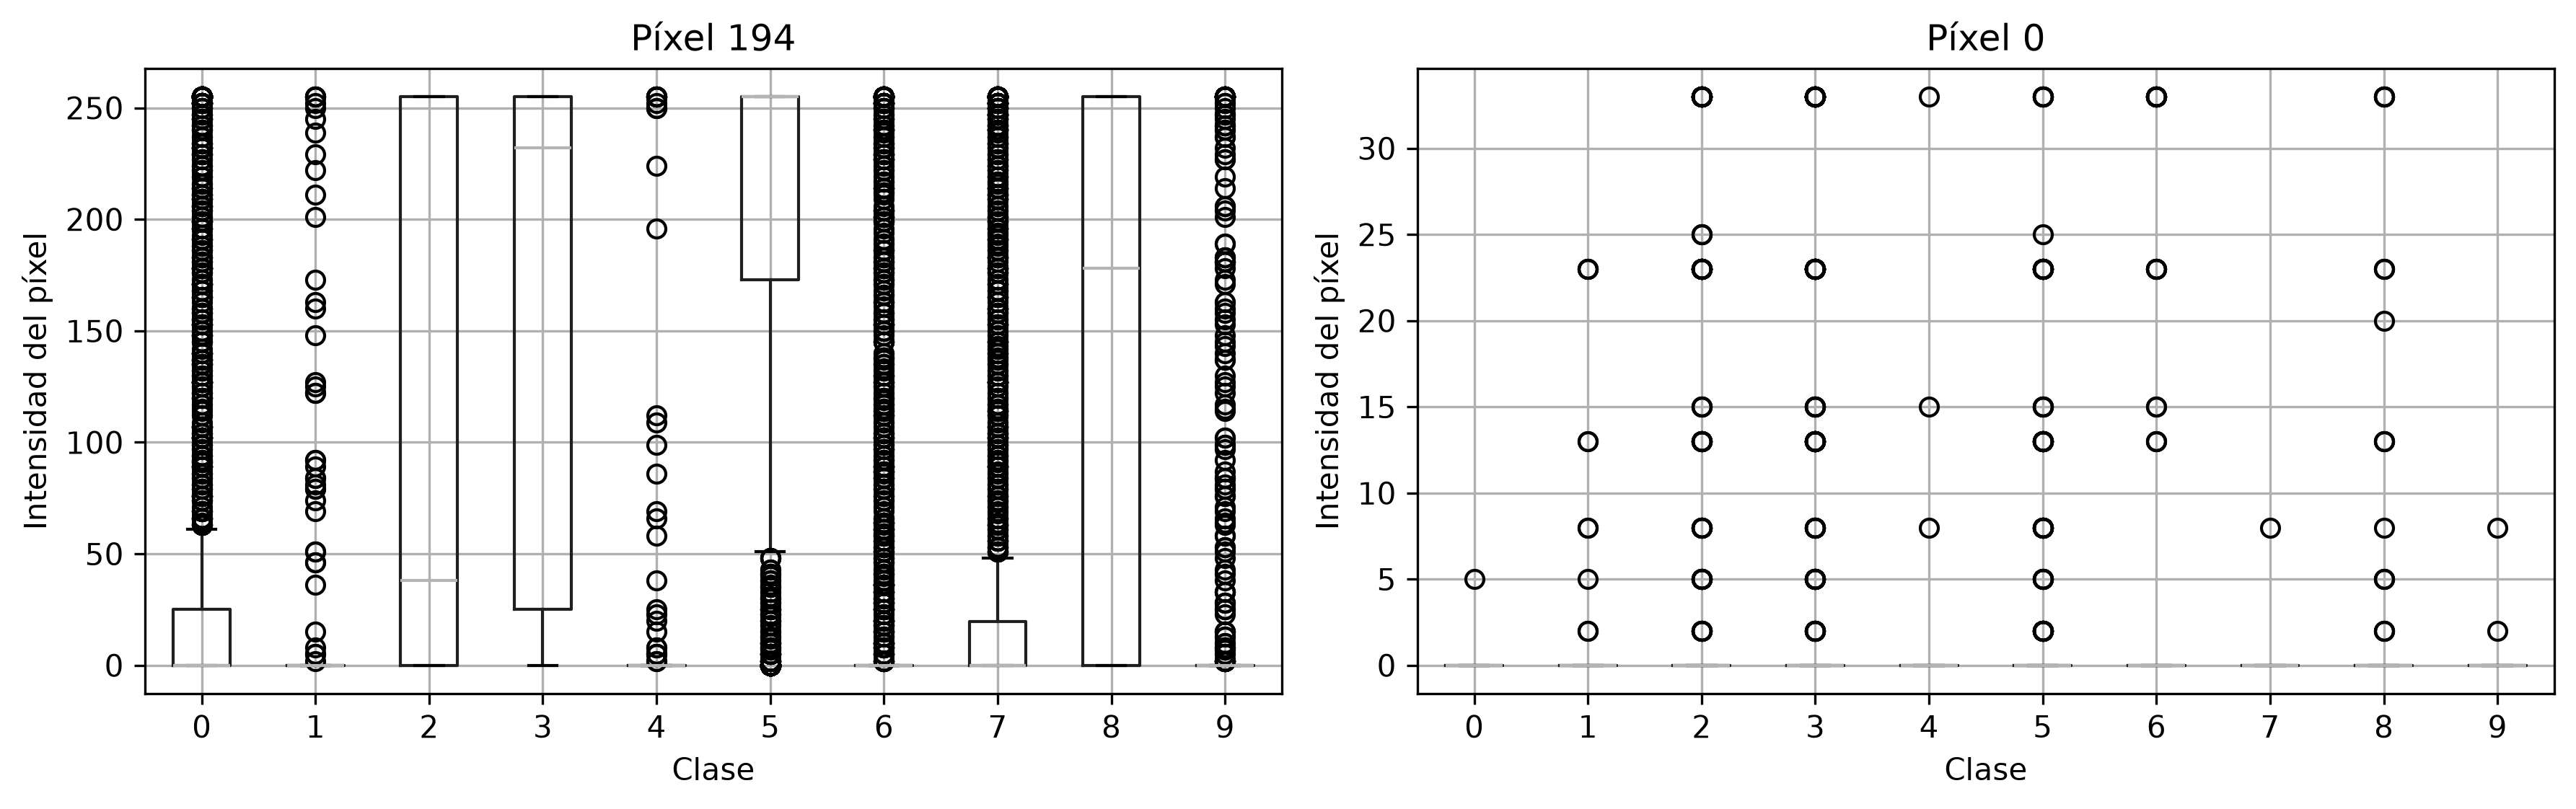
\includegraphics[width=0.85\textwidth]
    {graficos/comparacion_pixeles.png}
    \caption{Distribución de las intensidades de los
    píxeles 194 y 0 según la clase de la imagen.}
    \label{fig:comparacion_pixeles}
\end{figure}

Para complementar el análisis estadístico, seleccionamos
aleatoriamente ejemplos de las cuatro clases estudiadas
en los siguientes apartados: cuadrados, casas, estrellas
y peces.

La inspección visual de estos dibujos permite apreciar
las diferentes formas en que puede representarse una
misma categoría y contextualizar las medidas de
variabilidad y distancia utilizadas posteriormente.

\begin{figure}[H]
    \centering

    % Primera fila: cuadrados y casas
    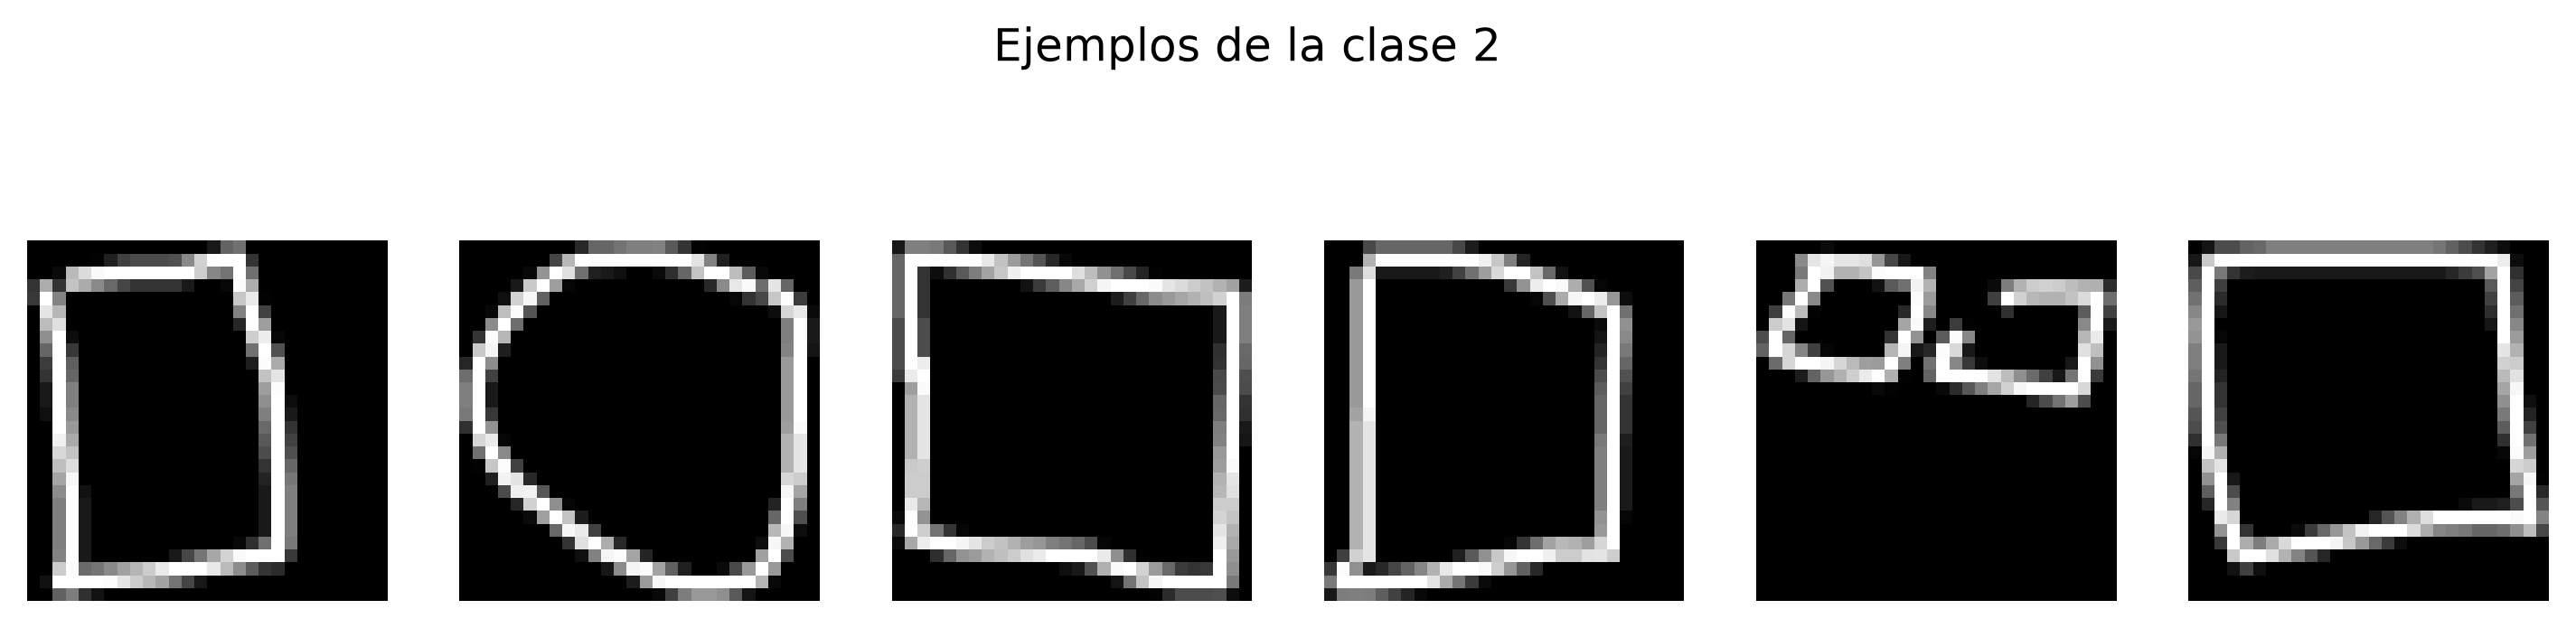
\includegraphics[width=0.47\textwidth]
    {graficos/ejemplos_de_clase_2.png}
    \hfill
    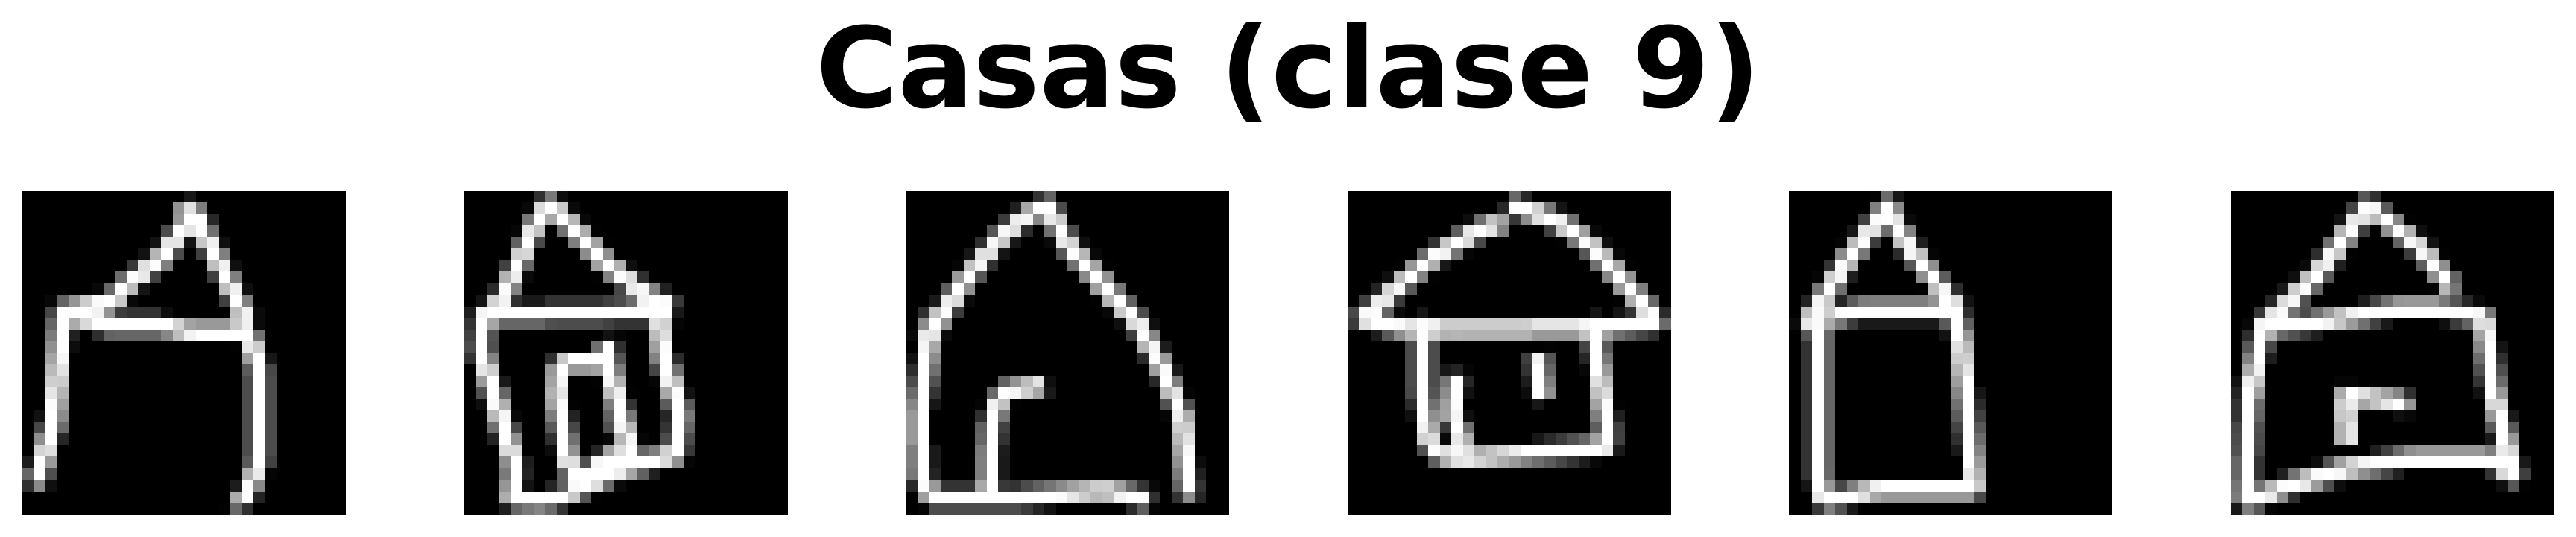
\includegraphics[width=0.47\textwidth]
    {graficos/ejemplos_de_clase_9.png}

    \vspace{0.3cm}

    % Segunda fila: estrellas y peces
    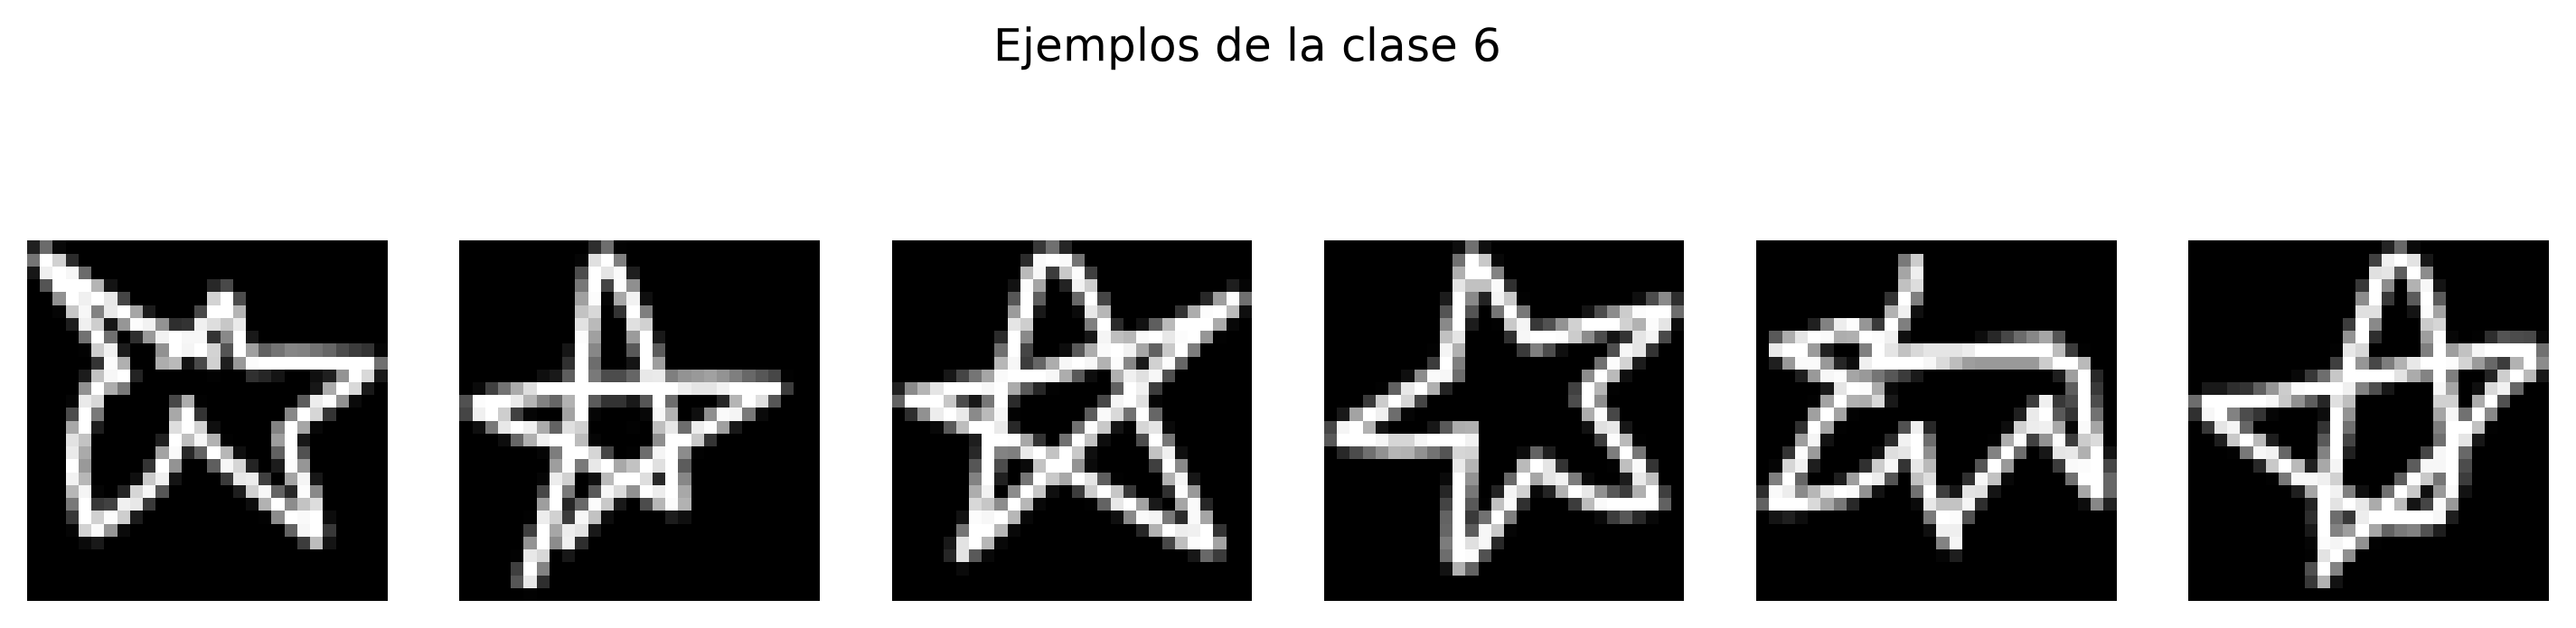
\includegraphics[width=0.47\textwidth]
    {graficos/ejemplos_de_clase_6.png}
    \hfill
    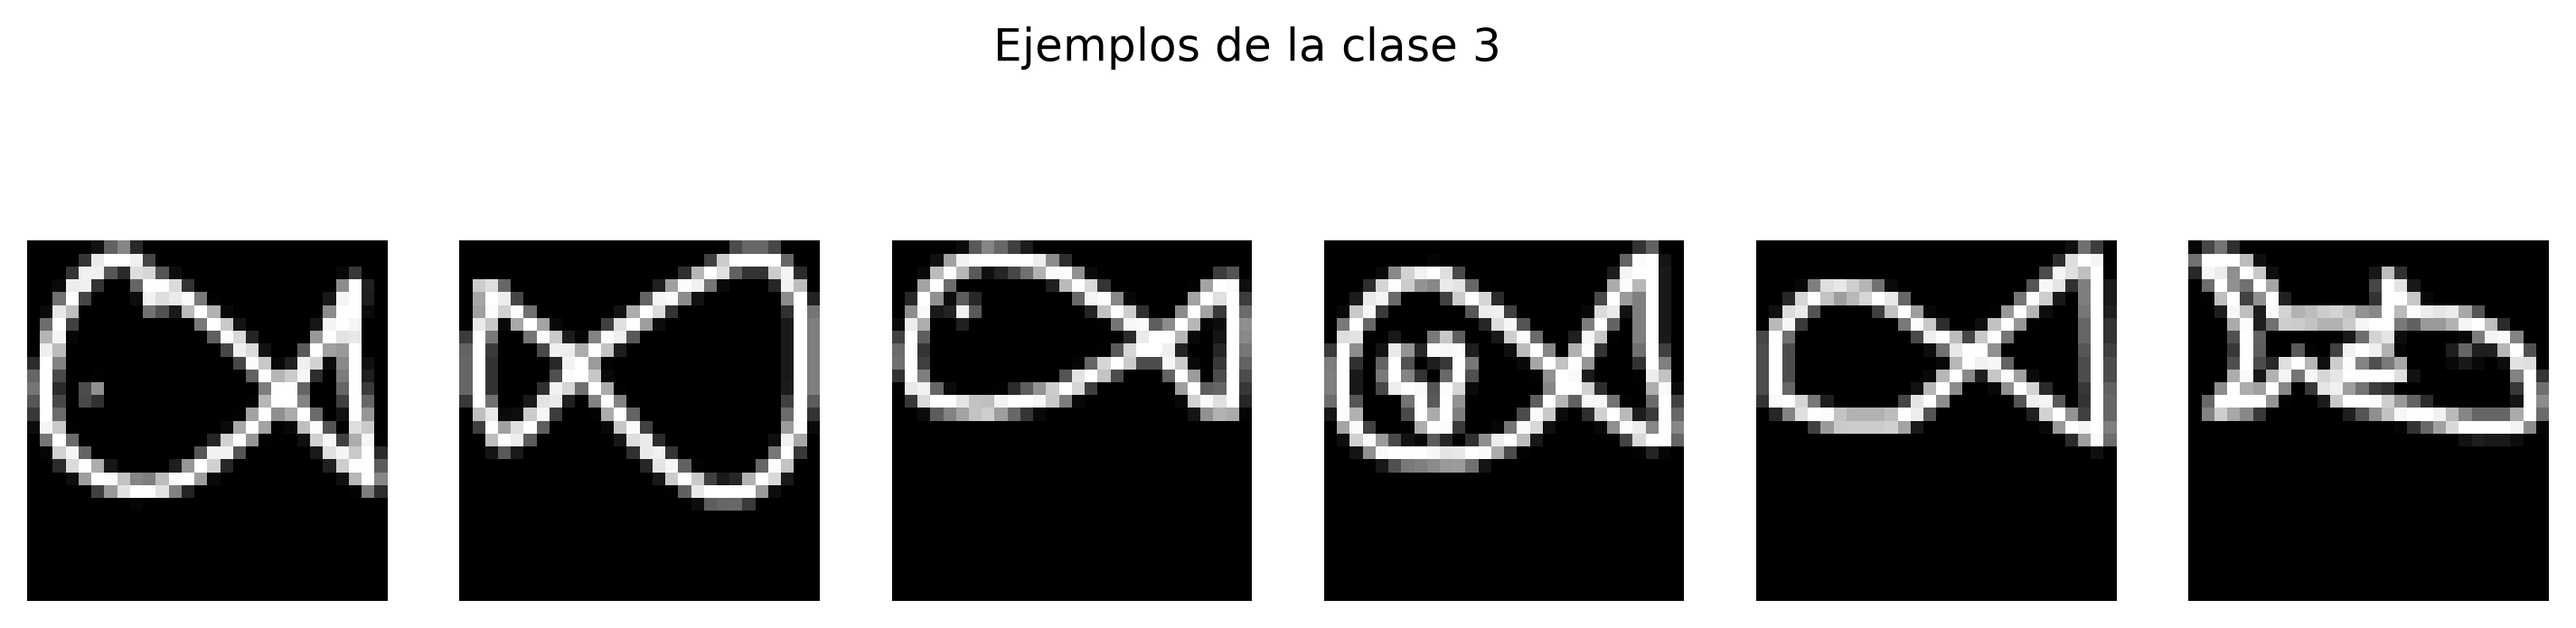
\includegraphics[width=0.47\textwidth]
    {graficos/ejemplos_de_clase_3.png}

    \caption{Ejemplos de imágenes seleccionadas
    aleatoriamente de cuatro clases del conjunto
    de datos. Arriba: cuadrados (2) y casas (9).
    Abajo: estrellas (6) y peces (3).}
    \label{fig:ejemplos_clases}
\end{figure}

A continuación, analizamos las similitudes entre
imágenes de cuadrados (clase 2), estrellas (clase 6)
y casas (clase 9). Para ello, seleccionamos aleatoriamente
100 imágenes de cada categoría y calculamos las distancias
euclídeas tanto entre imágenes de clases diferentes como
entre imágenes de una misma clase.

A partir de la Figura \ref{fig:distancias_clases},
observamos que los cuadrados presentan las menores
distancias internas, con una mediana de 2900,37,
por lo que constituyen la clase más homogénea de las
tres analizadas según esta medida. En cambio, las estrellas
y las casas presentan medianas de 3240,39 y 3194,37,
respectivamente, lo que refleja una mayor dispersión
entre sus representaciones.

En cuanto a las distancias entre clases diferentes,
encontramos que la mayor distancia media corresponde
a cuadrados y estrellas (3502,25), seguidos de casas
y estrellas (3369,07) y cuadrados y casas (3326,96).
Por lo tanto, los cuadrados y las estrellas presentan
las mayores diferencias promedio según la distancia
euclídea utilizada.

No obstante, observamos un solapamiento considerable
entre las distribuciones de distancias internas y
entre clases. Esto nos permite reconocer diferencias
en la homogeneidad y separación de las categorías,
pero no determinar por sí solo cuáles resultarán más
fáciles de distinguir mediante un clasificador.

Además, debemos considerar que la distancia euclídea
compara las intensidades de los píxeles en posiciones
correspondientes. En consecuencia, dibujos visualmente
similares pueden presentar distancias elevadas si
difieren en su ubicación, tamaño u orientación.

\begin{figure}[H]
    \centering
    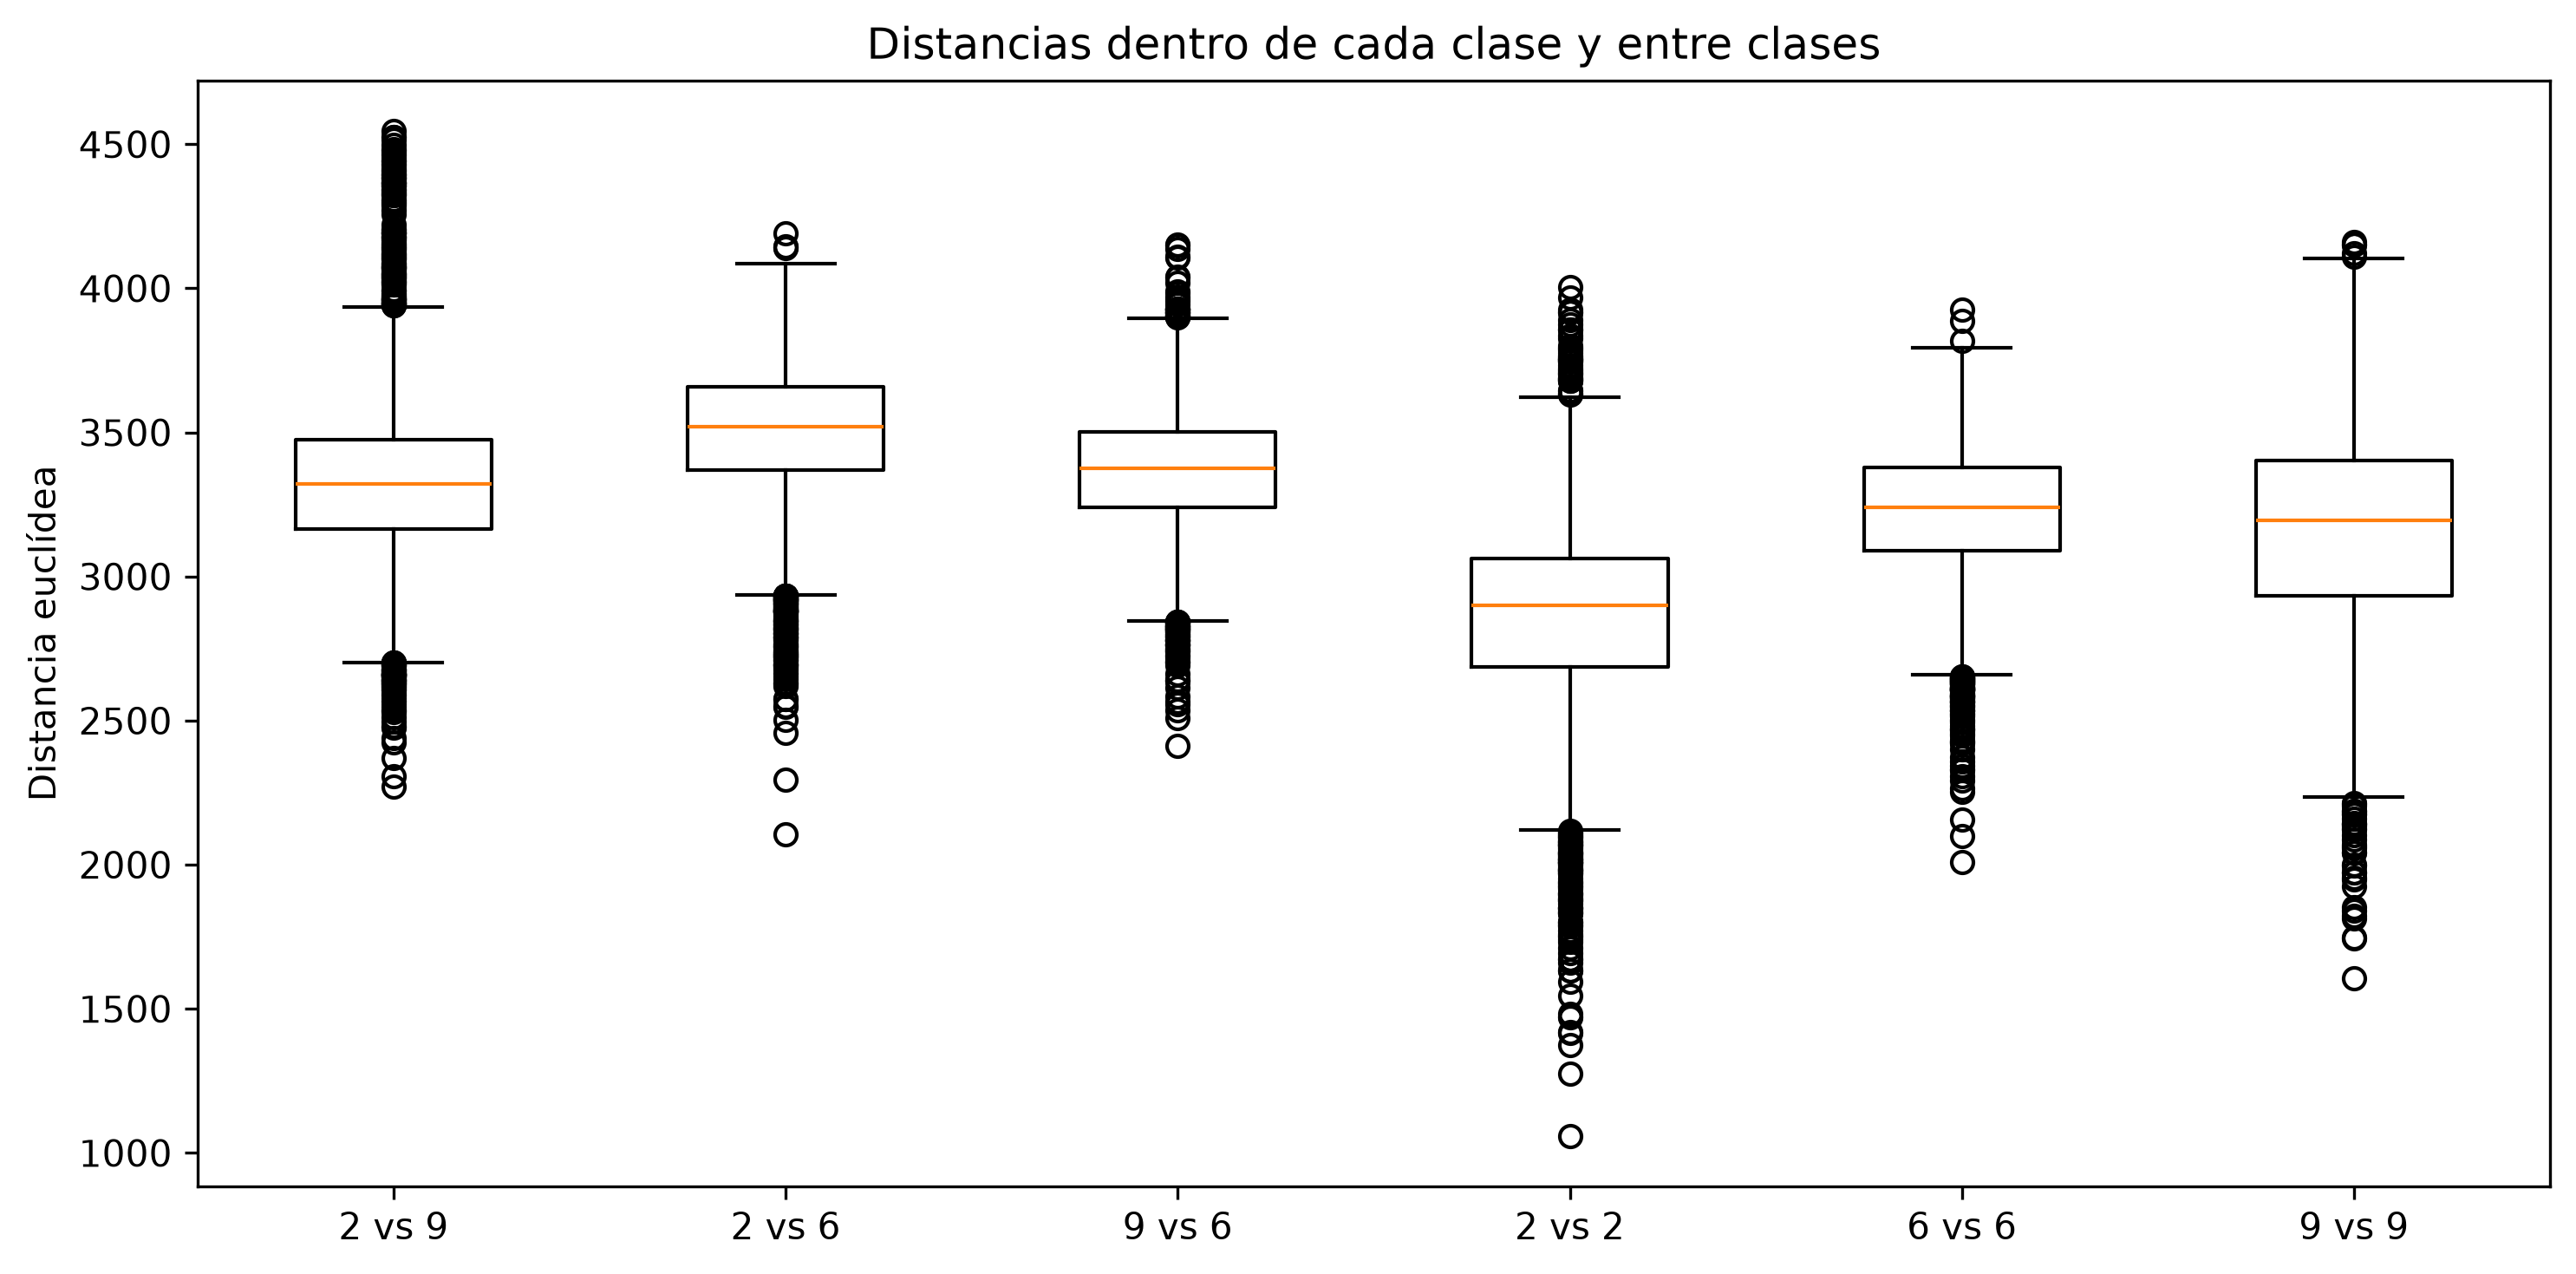
\includegraphics[width=0.85\textwidth]
    {graficos/distancias_clases.png}
    \caption{Distribución de las distancias euclídeas
    entre imágenes de una misma clase y de
    clases diferentes.}
    \label{fig:distancias_clases}
\end{figure}

Por último, estudiamos la similitud entre las imágenes
de la clase 3 (peces). Para ello, construimos una imagen
promedio a partir de las intensidades medias de sus
píxeles y un mapa de desvío estándar que nos permitió
visualizar la variabilidad interna de la categoría.

Como se observa en la Figura
\ref{fig:variabilidad_peces}, la imagen promedio presenta
una forma difusa, lo que sugiere diferencias entre las
representaciones de los peces. Por otra parte, notamos
que la mayor variabilidad se concentra en la región
superior y los laterales de las imágenes, mientras que
la región inferior presenta valores considerablemente
menores.

\begin{figure}[H]
    \centering
    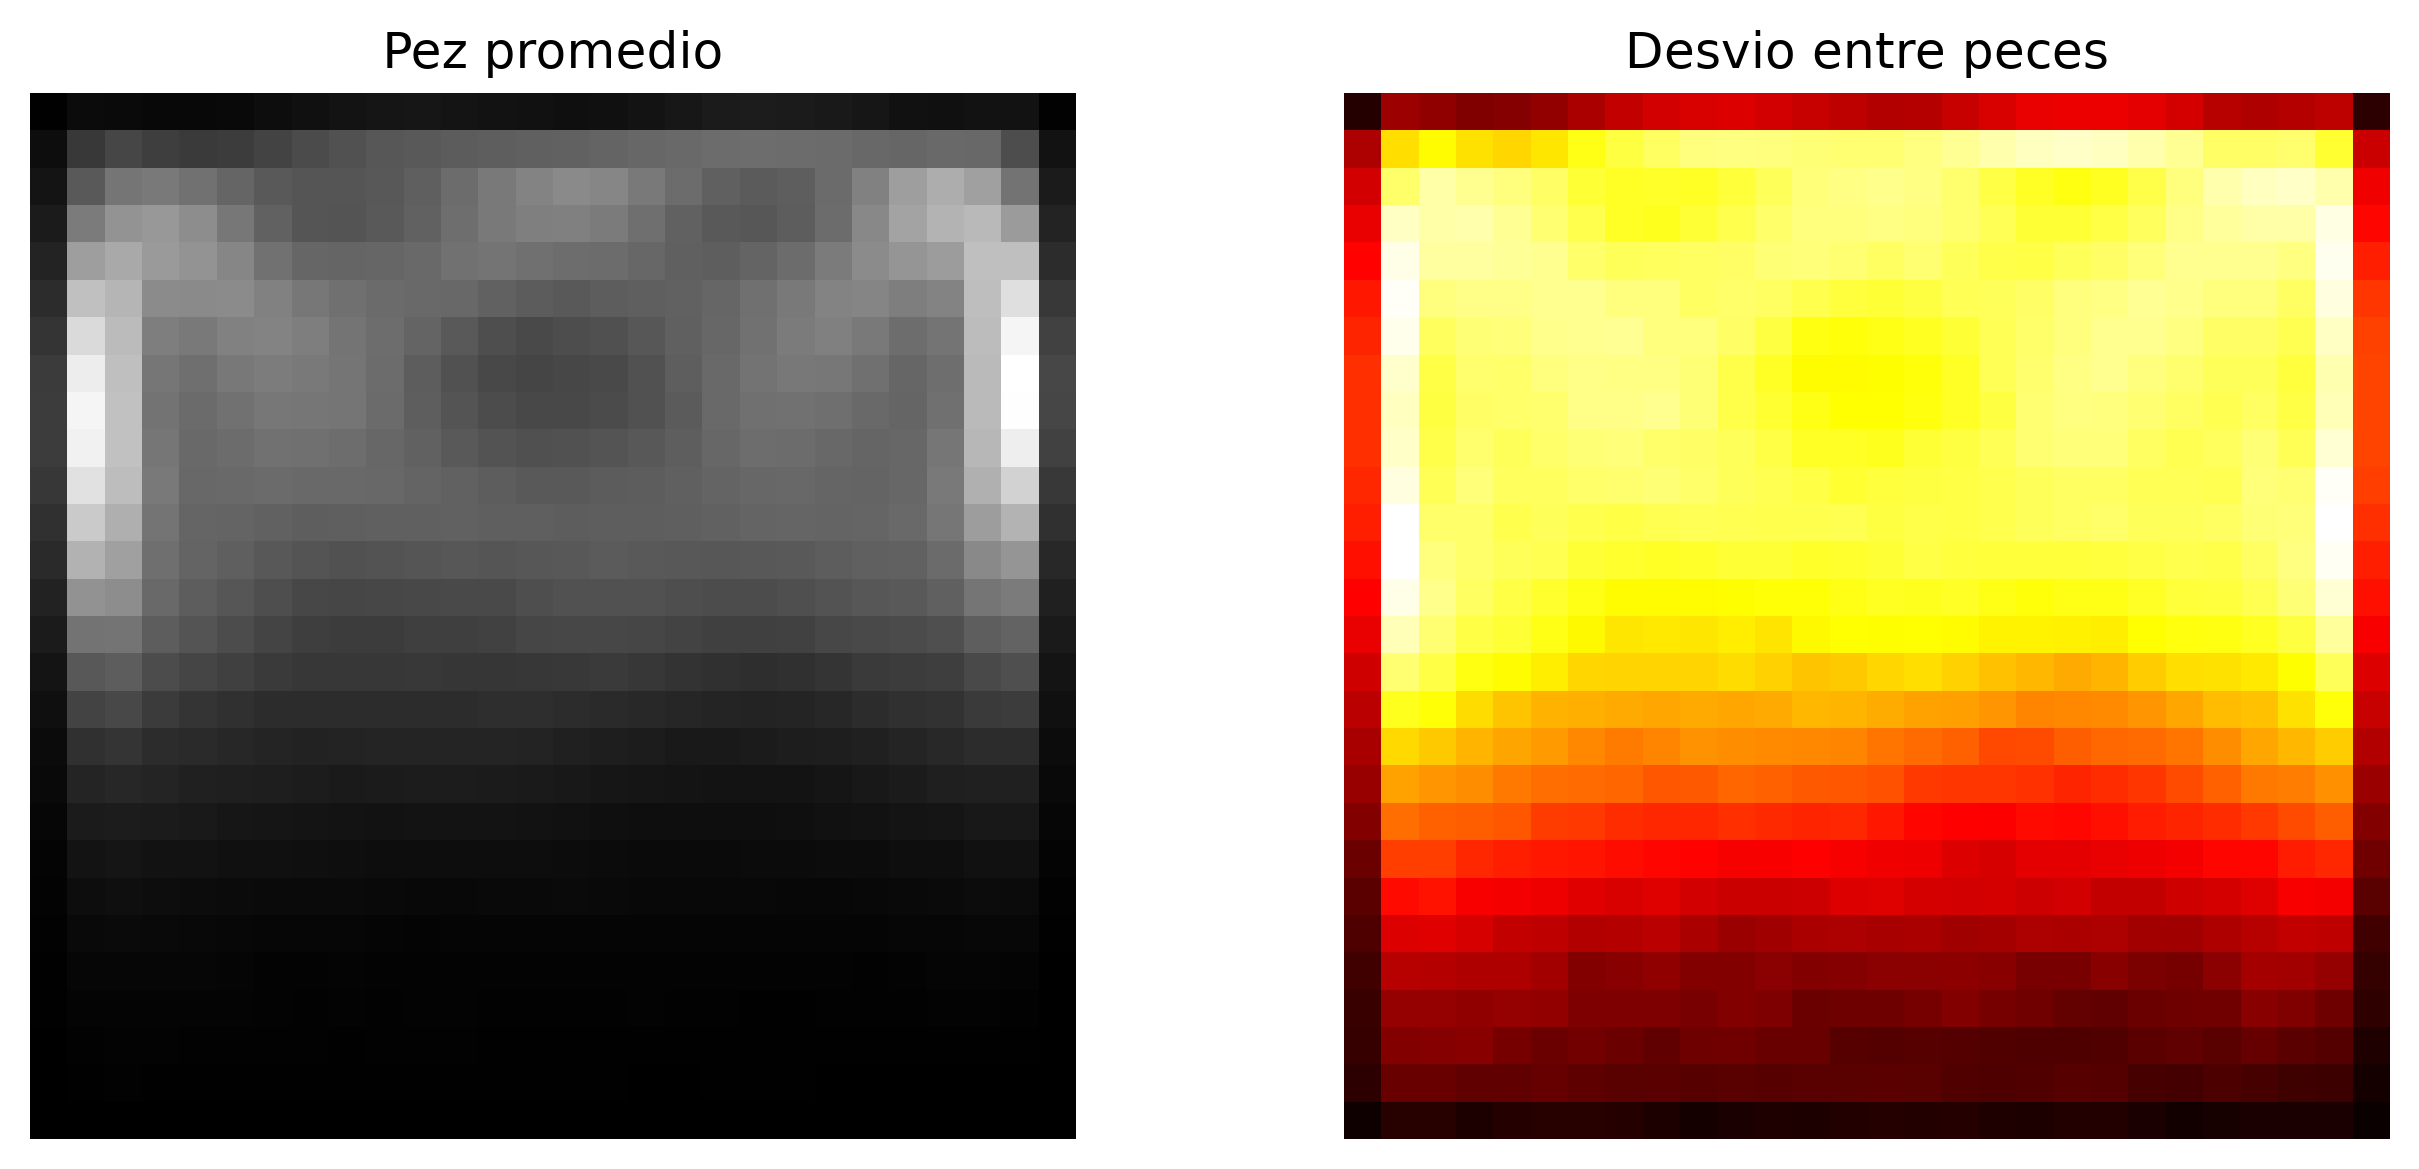
\includegraphics[width=0.8\textwidth]
    {graficos/peces_promedio_desvio.png}
    \caption{Imagen promedio y desvío estándar
    por píxel de la clase 3 (peces).}
    \label{fig:variabilidad_peces}
\end{figure}

Para complementar estas observaciones, comparamos
las distancias euclídeas entre pares de peces,
entre peces y cuadrados y entre pares de cuadrados.

En la Figura \ref{fig:distancias_peces} observamos que
las distancias internas entre peces presentan una
mediana cercana a 2900, ligeramente inferior a la
distancia mediana entre peces y cuadrados, próxima
a 3120. Sin embargo, las distribuciones se solapan
considerablemente y las distancias internas de peces
y cuadrados son similares.

Por lo tanto, encontramos variaciones apreciables
entre las representaciones de peces, aunque su
dispersión interna no resulta particularmente elevada
en comparación con la de los cuadrados, según la
distancia empleada. Estas observaciones no permiten
determinar por sí solas qué tan fácilmente pueden
clasificarse las imágenes de esta categoría.

\begin{figure}[H]
    \centering
    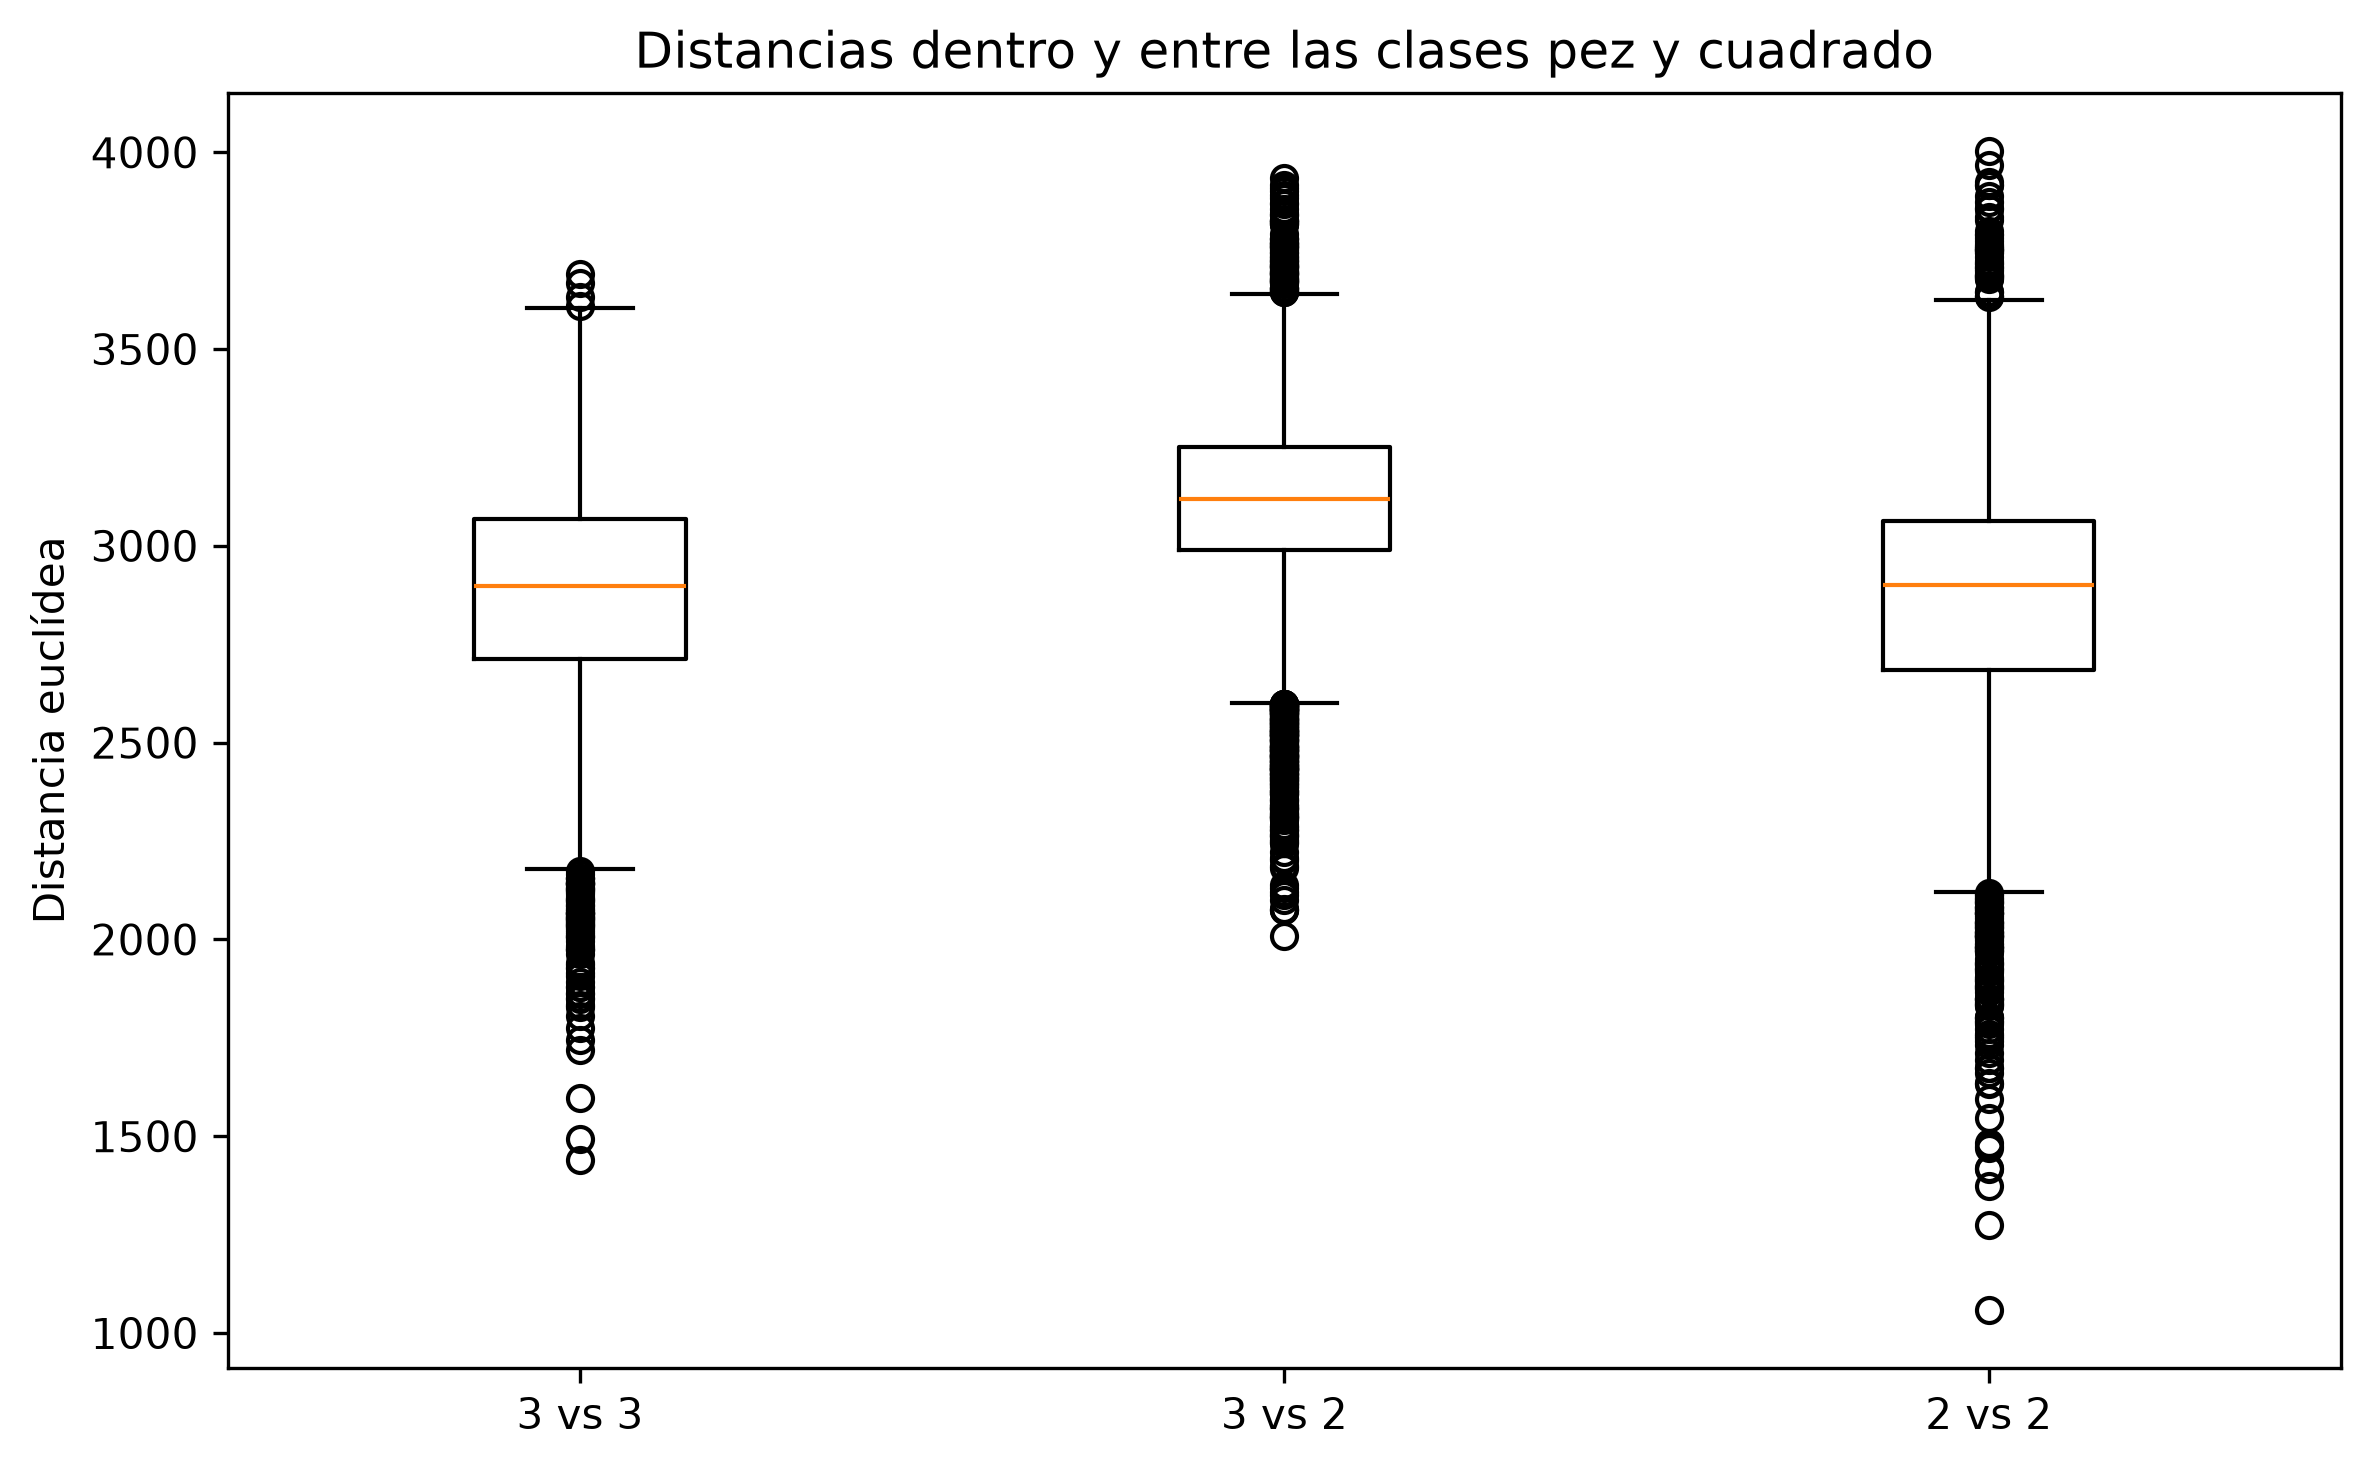
\includegraphics[width=0.75\textwidth]
    {graficos/distancias_peces.png}
    \caption{Distribución de las distancias euclídeas
    dentro de las clases 3 y 2, y entre ambas clases.}
    \label{fig:distancias_peces}
\end{figure}

El análisis exploratorio de imágenes presenta dificultades asociadas a su 
alta dimensionalidad y a la importancia de la disposición espacial de los píxeles.
El estudio individual de las intensidades no permite recuperar completamente las formas 
de los dibujos, mientras que diferencias en la posición, el tamaño o la orientación pueden 
generar variaciones importantes dentro de una misma clase.

Para abordar estas dificultades, combinamos herramientas estadísticas y visuales que nos 
permitieron identificar patrones de variabilidad y similitud. Sin embargo, estos resultados 
no permiten determinar por sí solos la capacidad predictiva de los atributos ni la separabilidad 
de las clases. Por ello, en los siguientes ejercicios evaluamos empíricamente el desempeño de 
distintos clasificadores y cómo este cambia según los atributos e hiperparámetros seleccionados.

% ==================================================
\section{Experimentos realizados}
% ==================================================

En esta sección se describen los experimentos realizados,
las decisiones tomadas durante el desarrollo y los resultados
obtenidos. Para cada experimento se especifican el objetivo,
la metodología y las observaciones principales.

\subsection{Preparación de los datos}

Antes de entrenar los modelos, se realizó [describir el
preprocesamiento aplicado]. Se utilizaron los conjuntos de
datos de entrenamiento y evaluación según lo establecido
en la consigna.

Las decisiones de preparación de los datos se tomaron
considerando [justificar brevemente las decisiones relevantes].

\subsection{Primer experimento: [nombre del experimento]}

El objetivo de este experimento fue [objetivo].

Para realizarlo, se utilizó [modelo o método], con
[describir brevemente la configuración y los parámetros
más importantes].

Los resultados obtenidos fueron [incluir resultados
relevantes y métricas]. A partir de ellos, se observó que
[interpretar el resultado, sin limitarse a repetir los valores].

% Insertar el gráfico si aporta información.
%
% \begin{figure}[H]
%     \centering
%     \includegraphics[width=0.75\textwidth]{imagenes/experimento1.png}
%     \caption{Resultados del primer experimento.}
%     \label{fig:experimento1}
% \end{figure}

\subsection{Segundo experimento: [nombre del experimento]}

En este experimento se buscó [objetivo], modificando
[parámetros, atributos o modelo respecto del experimento
anterior].

Se obtuvo [resultados principales]. La comparación con
el experimento anterior permite observar que [interpretación
de las diferencias].

% Agregar subsecciones para los experimentos que realmente
% se hayan realizado, sin repetir información innecesaria.

\subsection{Comparación de resultados}

Para comparar los modelos y configuraciones evaluados,
se resumen los resultados principales en la Tabla
\ref{tab:resultados}.

\begin{table}[H]
    \centering
    \caption{Comparación de los experimentos realizados.}
    \label{tab:resultados}
    \begin{tabular}{lcc}
        \toprule
        Experimento & Métrica utilizada & Resultado \\
        \midrule
        Experimento 1 & [métrica] & [valor] \\
        Experimento 2 & [métrica] & [valor] \\
        Experimento 3 & [métrica] & [valor] \\
        \bottomrule
    \end{tabular}
\end{table}

Los resultados muestran que [resumir qué configuración
obtuvo el mejor desempeño y qué diferencias relevantes
se encontraron].

% ==================================================
\section{Conclusiones}
% ==================================================

A partir de los experimentos realizados, se concluye que
[resumir los principales hallazgos del trabajo].

En particular, el modelo [nombre del modelo] obtuvo
[resultado relevante], mientras que [otro modelo o
configuración] presentó [resultado]. Estas diferencias
pueden explicarse por [justificación basada en los
experimentos y las características de los datos].

Respecto del inciso 3.e, la accuracy estimada fue de
[valor o porcentaje]. Esta estimación se obtuvo mediante
[método utilizado para estimarla], utilizando
[describir los datos o particiones empleados].

La estimación resulta razonable porque [justificar a partir
del procedimiento de evaluación, los resultados obtenidos
y las limitaciones que correspondan]. Sin embargo, debe
tenerse en cuenta que [mencionar posibles limitaciones,
incertidumbre o diferencias entre los datos utilizados
para evaluar y los datos finales].

En síntesis, los resultados permiten afirmar que
[conclusión final directamente respaldada por los
experimentos realizados].

% ==================================================
\section{Bibliografía}
% ==================================================

\begin{thebibliography}{9}

\bibitem{paper}
[Autores del paper].
\textit{[Título completo del paper]}.
[Revista, congreso o publicación, año].
[DOI o URL, si corresponde].

% Agregar las demás fuentes consultadas.
% Ejemplo de documentación:
%
% \bibitem{documentacion}
% Scikit-learn.
% \textit{Documentación oficial}.
% \url{https://scikit-learn.org/stable/}

\end{thebibliography}

\end{document}


